\section{Cybersecurity modelling as multiagent systems}
\label{sec:multiagent}
\subsection{Overview}
The same infrastructure and abstractions for programmatically defining security model parameters could perhaps be leveraged more easily in different environments. A few major drawbacks involve performance and data analytic solutions that become harder to work with in the Haskell environment. We are limited to the realm of rational verification, without explicit security guarantees that can be easily implemented into real-world deployments. Developing a layer to bridge game-theoretic solution concepts to address real-system defensive mechanisms remains as a problem in its own right. Moving towards reinforcement learning techniques to develop dynamic models, the open-game-engine needs more development. Additionally, we would be saddled with developing data structures for applications such as enterprise computer networks (i.e. directed graphs) which may be unwieldy to work with compared to other languages such as Python. In the same vein of compositionality at the user/modeller level, perhaps using a model-checking paradigm as our engine for verification allows for more tractable solutions. In this chapter, we present our findings investigating an approach to cybersecurity model verification by integrating two tools: VITAMIN and CyberBattleSim. 
\subsection{Discussion on rational verification}

The most recent work that uses software-assisted tools for Stackelberg security games is \cite{Phetmanee2024}, using rational verification. Rational verification is a formal-analysis technique for determining the equilibrium properties of multiagent systems. Specifically by encoding these properties in Linear Temporal Logic, practitioners can use model-checkers such as PRISM to verify that given models satisfy properties. After writing these propositions, PRISM can act as an equilibrium checker by checking all possible states of the game. In particular, \cite{Phetmanee2024} extends the PRISM framework to demonstrate the security properties detailed in CVE-2017-8759, and generates data demonstrating the defensive conditions and recommendations for security advisors. 


By using the PRISM-model checker and the PRISM property-specification language, it has been shown that security games can be mechanically verified. More recent work has extended PRISM to handle Stackelberg equilibrium for security games \cite{Phetmanee2024}. The complete software for two example models can be found at \cite{phetmanee_2024_13338608}. According to the proposed worfklow, there are automated tools to translate CVEs to attack-defense trees to Stackelberg Security Games, defined as a data structure storing the extensive-form representation of the game and atomic propositions that encode the reward structure as dictated in the attack-defense tree. For future work, encoding attack-defense trees defined in other models to be compatible with supplying payoffs in open games would be an interesting direction.

However, the models developed in \cite{Phetmanee2024} aren't built expressively for the reason of further extensionality in the future. The deliverable allows a user to provide a specific CVE and attacker action as a logical formula, and line-by-line entries for associated costs for specific attacker or defender actions. Finally, a security expert can input a certain patch or security property to test for Stackelberg equilibrium and whether that security property can be satisfied. 

The output of the StEve tool and the open-games diagnostic info are similar in terms of displaying each players associated payoff. However, the open-games-engine doesn't prove any satisfiability constraints, it's up to the modeller to check all possible states, whereas PRISM will be able to compute equilibrium automatically. Thus, StEve requires less understanding from security experts for running the game model, but prevents any amendments to game structure, such as an attacker being first-to-act rather than the defender. Working in the open-games environment necessitates more direct construction of the game with at most the import of the security games provided as a template in this thesis, but allows for greater maneuverability.

Comparatively, working in Haskell vs PRISM comes with the advantage of a type checker and various other language tools that will be expounded upon in the following chapter. An example difference is not needing to translate into a temporal logic formulae, but writing property tests using Hspec. The perceived downside is the inherent difference in computational complexity and running time for these models, which has yet to be determined. But from a useability point-of-view, a modeller can programmatically generate different attack or defense strategy profiles to test for any given model, with the tradeoff of not having a compact logic to run through the usual model-checking techniques. 

\subsection{Preliminaries}
Model-checking is a verification technique for ensuring that systems meet their requirements and specifications. We can do this by examining the system's representation as a model $\mathcal{M}$ and the representation of the desired specification as a formula $\phi$ in a logical system such as linear temporal logic (LTL) (we refer readers to \cite{baier2008principles} for a wide-scope view of model-checking). To follow the interaction between many rational agents taking actions over this model, we are tasked with the verification of a multi-agent system (MAS).

We first recall the definition of an obstruction model given in \cite{catta2024obstruction}


\begin{definition}[Concurrent game structure]
Given a (countable) set of atomic propositions $Ap$ and a set of agents $Ag$ ${1, ... k}$, a \textit{concurrent game structure} over $Ap$ and $Ag$ is a tuple
$\mathcal{C} = (S, s_{I}, Act, P, T, \mathcal{V})$ where
\begin{itemize}
    \item $S$ is a non-empty set of states;
    \item $S_{I}$ is the initial state;
    \item $Act$ is a finite, non-empty set of actions;
    \item $P: S \times Ag \rightarrow 2^{Act}/ \emptyset$ is the protocol function that gives all the actions that an agent $i$ is allowed to take to at a given state $s$;
    \item $T: S \times J \rightarrow S$ is the (partial) transition function that is defined for state $s$ and joint action $\mathbf{a}$ if for every $i \in Ag, \mathbf{a}(i)\in P(s,i)$ J is the set of maps from $Ag$ to $Act$, which denotes joint actions i.e. $\mathbf{a}$, $\mathbf{b}$;
    \item $\mathcal{V}: S \rightarrow 2^{Ap}$ is the valuation function that gives to every state $s \in S$ a subset of $Ap$ that are true at $s$.
\end{itemize}
Combined with a cost function $\$: S \times J \rightarrow \mathbb{N}^{+}$, we can construct a directed, weighted graph as an obstruction model, written as a tuple $\mathcal{M} = (\mathcal{C}, \$ )$. The edges of this graph are labeled by joint actions, and weighted according to the cost function $ \$ $
\end{definition}

Note we call this an \textit{obstruction} model precisely because we give a specific player (a \textit{Demon} or simply defender agent for our purposes) the capability of dynamically changing this graph by removing edges. The defender agent will remove edges according to a specific strategy, thereby temporarily restricting the set of actions the attacker can take at each state. We call a finite sequence of states $\pi_{1}, \pi_{2} ... \pi_{i} \text{ for any } i \in \mathbb{N}^{+} \text{ s.t } \exists \mathbf{a}\in J, \pi_{i+1} = T(\pi_{i}, \mathbf{a})$ a \textit{history} $\mathbf{h}$. We use $last(\mathbf{h})$ to denote the last state of the sequence. For any state $s\in S$, we say all the possible joint actions that can be taken at the state as the set $J(s) = \{\mathbf{a}\in J \, | \, T(s, \mathbf{a}) = s' \text{ for some } s' \in S\}$

\begin{definition}[Demonic n-strategy] For an obstruction model $\mathcal{M}$ and $n \in \mathbb{N}$, a \textbf{demonic n-strategy} is a function $\mathcal{G}: H \rightarrow 2^{J}$ which for any history $\mathbf{h}$ gives a subset $A_{\mathcal{G}} \subset J(last(h))$ and $(\Sigma_{\mathbf{a}\in A_{\mathcal{G}}}\$ (last(h), \mathbf{a})) \leq n$
\end{definition}

Thus the defender strategy selects $A_{\mathcal{G}}$, a subset of all the possible joint actions at for some history $\mathbf{h}$.

\subsection{CyberBattleSim}
\label{sec:CyberBattleSim}
CyberBattleSim \cite{msft:cyberbattlesim} is a research-experimentation software for modelling a wide-range of cybersecurity situations. This platform gives users flexibility in defining use-cases with fine-tuned parameterization, ranging from complex enterprise-network intrusion situations to simple Capture-the-Flag simulations.\cite{ccyberbattle} integrates this platform with active data scraping techniques to populate the simulation environment with real-world vulnerabilities from the NVD database \cite{booth2013national}. However, CyberBattleSim currently only supports active (learning) attacker agents, whereas defender agents are static, probabilistic actors of the simulation.
\subsection{Mechanism}
CyberBattleSim gives users the functionality for instantiating an OpenAI Gym environment for which an attacker agent, following various reinforcement learning algorithms, will traverse this environment. The attacker agent maintains a (private) internal state representing its view of this environment at each timestep, accumulating credentials and rewards for each attempted exploits. As expected, the attacker agent's primary goal is to maximize this reward by traversing the network topology of this environment through exploits. At each step of the simulation, the validity of an attempted exploit is handled accordingly. For example, while the observation space of the attacker may include an \textit{AzureStorage} node, but the attacker does not have the necessary cached credentials acquired from previous exploits, so a negative reward will be given and the outcome of the attempt is a fail-restart outcome.

The outcomes of available actions at any given timestep is determined by this internal state. There are three actions an attacker can take:
\begin{enumerate}
    \item Remote exploit: from a currently-owned source node, execute a remote vulnerability existing on another node
    \item Local exploit: on a currently-owned node, execute a local vulnerability existing on that node
    \item Lateral move: using the proper gathered credentials from previous moves, gain ownership of a discovered node
\end{enumerate}

Lateral-move exploits are not required to be explicit when defining the vulnerabilities available at each node. On the other hand, all unique vulnerabilities assigned to a node of the network are either of type Remote or Local. Therefore a lateral-move exploit isn't tied to any specific vulnerability, but can be inferred as a possible action depending on the gathered credentials.

\subsection{Defender agent}
A CBS simulation can be optionally run with the inclusion of a probabilistic defender. This defender follows a static strategy that selects subsets of CBS nodes in the topology to reimage for a set number of timesteps. Reimaging shuts off the node, the services it's running, and removes an attacker's previous ownership of the node. The defender agent is assessed by the availability of the services provided by all the nodes, given a certain service-level agreement weighting depending on the importance of the service. Thus, reimaging one or many nodes has an associated cost to the defender.
\subsection{Usage and metrics}
From the modeller's perspective, she would write Python scripts (or Jupyter notebooks) to run these simulations and compare the performance of different attacker agents in a given environment. Modellers can then conduct baseline tests by experimenting with different learner implementations (see the \textit{learner} module and \textit{epsilon\_greedy\_search()}) and reading the statistics provided in the output log.

\begin{figure}[h]
\centering
\includegraphics[scale=0.2]{CBSStats.png}
\caption{Episode 10 output of evaluating an epsilon greedy search for a Deep Q-learning policy, with a static defender, from \textit{notebook\_withdefender.ipynb}}
\label{fig:stats}


\end{figure}

Note a modeller can use both the attacker's reward and improved reward over episodes, and the success rate for attempting different kinds of exploits. The simulation also comes equipped with a Plotly network topology trace representing the state of the network after the end of the simulation. The table in-between the Success Rate breakdown and the topology graph provides a textual snapshot of the attacker's known and discovered properties for each CBS node in the environment.

\subsection{Formal interpretation of the CyberBattleSim environment}
Now that we've established the current state-of-the-art for using CyberBattleSim, how do we design active defensive strategies for the defender? Following the model-checking paradigm, we need to construct and assess our interpretation of the network topology that hosts the attacker-defender-environment interaction in CyberBattleSim as an obstruction model.

\subsection{Identifying properties}
First, we notice that working in CyberBattleSim gives fine-tuned control over the parameterization of the details of the network we wish to model. Specifically, both in the manual and automated (C-CyberBattleSim) case, for each CBS node the following are given: \begin{enumerate}
    \item List of vulnerabilities, including a reference to exposed or accessible nodes via a specific vulnerability. Vulnerabilities are either of type \textit{local} or \textit{remote}
    \item List of properties such as stored credentials, type of service the node is hosting etc.
    \item The type of service that is running such as hosting a website or operating a firewall
    \item A status flag representing whether the node is running or not. This flag can only be set by defender actions by reimaging the node for $n$ timesteps, before the node is brought back up automatically
\end{enumerate}

Furthermore, we can determine a relation between each CBS node depending on whether the exploitation of a vulnerability on a node would provide some sort of access to another. For example, exploiting a vulnerability resulting in a \textit{LeakedCredentials} outcome would update the attacker's internal list of discovered nodes that it knows about (but does not own), thereby leaving this newly discovered node exposed to another vulnerability resulting in a \textit{LateralMove} outcome in the next timestep.

Thus, we can compute fer each possible attack by algorithmically searching through all valid exploits an attacker can make at each timestep. This is in contrast to allowing the attacker agent to exhaustively search through the environment space and updating its action space at each timestep accordingly. Similarly for the defender, which should be able to actively change the attacker's capabilities at each timestep, but with the added capability of having complete knowledge of the attacker's action space at each timestep. Note that every environment stores an empty graph, where nodes and edges are added depending on what actions the attacker takes on that environment. This graph is then used specifically for visualization purposes for simulation, to create edges that dynamically change according to the attacker's progress. \footnote{There are no attack-path trace capabilities yet, but would be an interesting direction to take for future research.}

Drawing from the case-study given in \cite{catta2024obstruction}, the defined attack graph gives nodes as the entire state of the system (all the CBS nodes), and edges representing the execution of an exploit. This falls would fall in-line with the information we can extract from the CBS simulation environment, but we need a way of determining the set of states of the CBS environment we want to explore. That is, we want the set of \textit{attacker-reachable} states of the CBS environment, where \textit{attacker-reachable} is a way of identifying whether there exists a sequence of vulnerabilities the attacker can exploit to reach that state. The following sections will formalize this idea by first defining an exploit-dependency graph $\mathcal{H}$ for each CBS environment and the corresponding vulnerabilities and exploit outcomes. Then, we'll use the set of attack paths of $\mathcal{H}$ to construct the set of states of an obstruction model.

For any given CyberBattleSim Gym environment, we'll denote the following static elements that are used at the top-level model instantation and to be used for remainder of the paper:
\begin{itemize}
    \item $N$ as the indexed set of (CBS) nodes of cardinality k, representing nodes in an enterprise network i.e. workstations, servers etc. For convenience we can refer to CBS node $n_{i} \in N \,  \forall i \, s.t. 1 \leq i \leq k $
    \item $Creds$ is the set of credentials that are present within the system. In CBS, each credentials are given by a string identifier along with the target CBS-node and access port.
    % \item $\mathcal{G} = (N,E)$ is the directed graph we'll use as a standard , where $E$ is the set of edges given by ordered pairs $\{(u, v) \in N \times N | \text{} \}$ We'll say that a successful outcome in CBS
    \item $Prop$ be the set of all string-valued properties in the system, used to identify an attacker's privilege level i.e. "Admin" or "LocalUser" or the status of a service i.e. "SSHOpen" or "WindowsRunning" on a CBS node. There is also a simple predicate-logic defined on this set given by the \textit{Precondition} class, where the symbols of an expression are properties in $Prop$. An example of a formula is "SSHOpen\&WindowsRunning"
    \item $Vulns$ is the set of vulnerabilities present in the simulation environment. Assume each vulnerability is unique and is associated with at least one CBS-node. Then we can define a function $\mathbf{getVulns}: N \rightarrow \mathcal{P}(Vulns)$ which selects a subset of vulnerabilities that are available to an attacker if they own the node the \textit{agent\_installed} flag is set to True. Each vulnerability has an optional \textit{Precondition} expression that states the prerequisite properties that the attacker must have already obtained or known before exploiting the vulnerability.

\end{itemize}
 Note that as mentioned in \ref{sec:CyberBattleSim}, lateral-move actions are not included in $Vulns$ because they are not instantiated explicitly. We can construct the set of possible lateral-move actions by satisfying the conditions:
 \begin{enumerate}
     \item Node-specific firewall rules of the target node allow the lateral move parameters i.e. if the lateral-move uses SSH, then the firewall of the target node must allow SSH traffic
     \item The attempted credential of the lateral-move must be in the set of allowed credentials for the service running on the target node
 \end{enumerate}

Using this, we can determine the set of all possible lateral-moves $Lats$ given by ordered pairs of nodes $(n_{i}, n_{j}) \in N \times N$ where target node $n_{j}$ satisfies the above conditions.

Putting this together, we define two functions over the total attack space $Vulns \cup Lats$. The function $\mathbf{getPreconds}: Vulns \cup Lats \rightarrow \mathcal{P}(Prop) \times \mathcal{P}(Creds)$ determines the necessary requirements to exploit a vulnerability, and $\mathbf{getPostconds}: Vulns \cup Lats \rightarrow \mathcal{P}(Prop) \times \mathcal{P}(Creds)$ returns the updated values of the properties of the system following the successful attack.
\subsection{Attack-path generation in CBS}

Rather than track the path of an attacker over the network topology, since a CBS node can be revisited any number of times, we can track the sequence of valid vulnerability exploits the attacker takes. For the purposes of generating an attack graph, we only want to consider vulnerability exploits resulting in a successful outcome, for example without errors pertaining to invalid credentials or targeting a non-existent node. In code, this is handled through the function \textit{process\_outcome} in the \textbf{actions.py} module. Since there is no direct ad-hoc relationship between the vulnerabilities or sequences of vulnerabilities that result in successful outcomes, we must construct one. In CBS, the preconditions for a vulnerability comprise of a set of gathered credentials, proper ownership of necessary nodes, etc. We will say that all the conditions we want to consider for any vulnerability exploit (and lateral-move exploit) to be successful be the set $Conds = Cred \cup Perm \cup \mathcal{P}(N)$, where $\mathcal{P}(N)$ represents the set of CBS nodes that are owned or discovered by the attacker.

\begin{definition}[Exploit-dependency attack graph, from \cite{zenitani2023attack}]
    An \textit{exploit-dependency attack graph} is a connected, directed graph $\mathcal{G} = (E \cup C, R_{r} \cup R_{i})$ where
    \begin{itemize}
        \item $E$ is the set of exploits
        \item $C$ is the set of security conditions, $E \cap C = \emptyset$
        \item $R_{r} \subseteq C \times E$ is the require-relation
        \item $R_{i} \subseteq E \times C$ is the imply-relation
    \end{itemize}
\end{definition}

Note that the set of nodes of this graph designate two types, an \textit{exploit} node or \textit{condition} node. There are two types of conditions, \textit{initial} and \textit{intermediate}. Initial conditions is the subset of conditions where for all other conditions, there are no exploits that imply those conditions. In CBS, this corresponds to the the initial state of the environment before the attacker has made any moves. For a well-constructed model, the action space of the attacker at the first timestep should be nonempty, so the initial conditions must be satisfied by that first timestep. For each possible attacker action in CBS, we will only check that the minimum set of conditions needed to successfully carry out the action are satisfied before executing. This is exactly given by the optional \textit{Precondition} formula for that vulnerability.

\begin{construction}[CBS exploit-dependency graph]
    An exploit-dependency graph for a CBS environment is $\mathcal{H}=(Vulns \cup Lats \cup Conds, R_{i} \cup R_{r})$ where the require-relation is defined $(v, c) \in R_{r}$ if $c$ is a subset of the image of $\mathbf{getPreconds}(v)$. The imply-relation is defined similarly but over the image of $\mathbf{getPostconds}(v)$
\end{construction}
We use $Vulns \cup Lats$ as our set of exploit nodes since the choice of action of attacker at each timestep is selecting a vulnerability or attempting a lateral move and processing its effect on the environment.

\begin{definition}[CBS attack path]
    A (finite) CBS attack path is a subgraph of $\mathcal{H}$ such that the final node in the path is a condition node.
\end{definition}

Starting at the initial conditions of a given CBS attack path, we can traverse the subgraph until reaching a final condition node (dubbed goal condition in \cite{zenitani2023attack}) as a result of executing the sequence of vulnerability exploits. In this case, these postconditions correspond to a certain CBS environment with updated values of CBS node properties, attacker-knowledge of CBS nodes in the topology, and the attacker's gathered credentials.

We consider each vulnerability to be one-time-use and unique, thus there are no repeated exploit nodes in the path. In our implementation, we use \textbf{hashed\_attacker.py} as a wrapper class around the \textit{AttackerActions} class to uniquely identify each object by a hash of the elements of $Conds$. These properties are precisely (1) tuple of discovered and owned CBS nodes, (2) tuple of gathered credentials $Creds$ (4) tuple of properties $Prop$. The wrapper class also exports an exhaustive depth-first search function over all the possible attacks a player can make at each timestep while exploring the CBS environment.

% Formally: let
% $\forall v \in Vuln \cup Lats, \forall c \in Conds \cup Perm \cup Creds \text{ such that } (v, c) \in R_{r}$

It is clear that the number of possible CBS attack paths is at least as large as the possible set of goal conditions that can be reached by allowing the attacker to take the sequence of actions dictated by the path. Note there could be many paths to reach the same goal condition (for example, two distinct vulnerabilities expose the same CBS node and provide the same credentials for that node). We call the set of all possible CBS attack paths as $\mathcal{K}_{\mathcal{H}}$.

% By using the \textit{hashed\_attacker.py} module, we can generate a hashed \textit{AttackerActions} object

\begin{mdframed}
\begin{example}[CBS attack paths of the ToyCTF environment]
\label{ex:attackpath}

A simple example included in CyberBattleSim is a manually-solved simulation found in \textit{notebooks/toyctf-solved.ipynb}. The network topology for the ToyCTF environment is defined in \textit{cyberbattle.samples.toyctf.toy\_ctf}, and we can give the following assignments:
\begin{itemize}
    \item $N$ = \{"client", "AzureVM", "AzureResourceManager[user=monitor]", "AzureResourceManager", "Sharepoint","AzureStorage", "GithubProject", "Website", "Website.Directory", "Website[user=monitor]"\}
    \item $Vulns$ =  \{"CredScan-HomeDirectory", "CredScanBashHistory", "SearchEdgeHistory", "AccessDataWithSASToken", "CredScanGitHistory", "ListAzureResources", "NavigateWebDirectory", "NavigateWebDirectoryFurther", "ScanPageContent", "ScanPageSource", "ScanSharepointParentDirectory"\}
    \item $Prop$ = \{"CTFFLAG:LeakedCustomerData", "CTFFLAG:LeakedCustomerData2", "CTFFLAG:Readme.txt-Discover secret data", "CTFFLAG:VMPRIVATEINFO", "GitHub", "MySql", "SasUrlInCommit", "SharepointLeakingPassword", "Ubuntu", "nginx/1.10.3"\}
    \item $Creds$ = \{"ReusedMySqlCred-web",  "monitorBashCreds", "azuread\_user\_credentials", "SASTOKEN1", "ADPrincipalCreds"\}
    \item $Lats$ = \{("client", "AzureStorage"), ("client", "Website"), ("client", "AzureResourceManager[user=monitor]"), ("client", "AzureResourceManager"), ("Website", "Website[user=monitor]") \}
\end{itemize}


Starting with the attacker only owning the "client" node at the beginning of the simulation, we can follow the sequence of actions of length 4 (SearchEdgeHistory, ScanPageContent, CredScanGitHistory, ("client", "AzureStorage")). See figure \ref{fig:toyctf} to see the result of the attacker's view of the network after executing this sequence. We can translate this to a CBS attack path as seen in figure \ref{fig:attackpath}. We follow the same methodology as in \cite{zenitani2023attack} where circular nodes are conditions and rectangular nodes are exploits. Note that the goal condition in this case is the "CTFFLAG:LeakedCustomerData" property being discovered.
\end{example}
\end{mdframed}
\begin{figure}[h]
\centering
\includegraphics[scale=0.5]{network.png}
\caption{Plotly trace graph from \textit{toyctf-solved.ipynb}}
\label{fig:toyctf}

\end{figure}

\begin{figure}
\label{fig:attackpath}
\centering
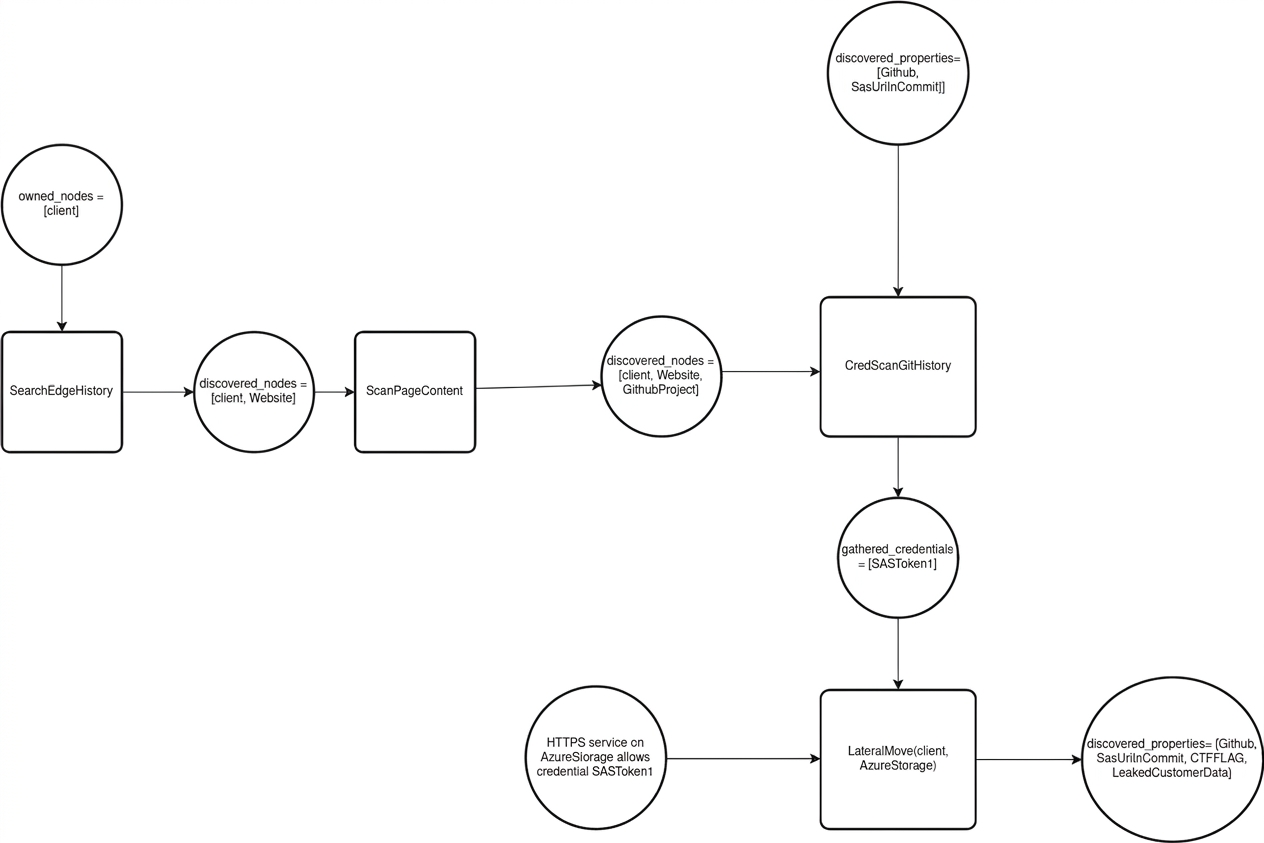
\includegraphics[scale=1.3]{images/attackgraphedited.jpg}

\caption{An example CBS attack path based on example \ref{ex:attackpath}}
\label{fig:attackpath}


\end{figure}


\subsubsection{Defender action cost module}
\label{sec:cost}
For edge-weights, since each edge is labeled by an exploit $v \in Vulns \cup Lats$, we can calculate the cost to the defender agent for preventing that vulnerability at each state. Let $\textbf{reimg}: Vulns \cup Lats \rightarrow \mathbb{N}$ be this weight-assignment function. For any CBS node $n_{i}\in N$, let the $j$-length tuple $(sla_{1}, sla_{2}, ... sla_{j})_{i} \in [0,1]^{j}$ giving the weights of each service $1 \leq k \leq j$, and $node\_sla_{i}$ is the weight of importance of the node relative to the total network availability. Since every vulnerability has some target CBS node $n_{i}\in N$,  we calculate the cost of reimaging the target node for that vulnerability by using the impact on the entirety of the network due to the loss of the services. Assume that the target node is operational (not already in a reimaging state). Let $X\subset N$ be the set of other CBS nodes that are currently in a reimaging state. Then deploying the next immediate countermeasure means the set of reimaging nodes is $X \cup \{n_i\}$. Finally,

\begin{align*}
\textbf{serviceWeight}(l) &= \begin{cases}
    0 & \text{if service } l \text{ is not running} \\
    \text{sla}_l & \text{if service } l \text{ is running}
\end{cases} \\[1ex]
\textbf{reimg}(v_i) &= \sum_{n_{l} \in N \setminus X \cup \{n_i\}} \text{node\_sla}_l \times \frac{1 + \sum_{1 \leq k \leq j} \textbf{serviceWeight}(k)}{1 + \sum_{1 \leq k \leq j} \text{sla}_k} \circ \textbf{targetNodeOf}(v_i)
\end{align*}



where $\textbf{targetNodeOf}: Vulns \rightarrow N$ returns the target node of the desired vulnerability exploit. Since the service weight tuples,   $node\_sla$ tuples, and the status of each service are all elements of $Conds$, we can lift our cost function to $\textbf{reimg}: Conds \times Vulns \cap Lats \rightarrow \mathbb{N}$ to match our desired type signature for weighting a concurrent game structure.
\newpage
\subsection{Deriving security objectives as atomic propositions}
Note that we specifically use \textit{Prop} to designate the system-wide properties. We would like to perform model-checking on these properties in VITAMIN. The VITAMIN input data does not necessitate any explicit interpretation of atomic propositions, just the labelling for each state and the label for each proposition. Fortunately, we can derive an interpretation for these labels using the information available in the CyberBattleSim environment. We can classify the properties of the environment into two parts: (1) model-wide and (2) node-specific. A model-wide property must be determined using one or more node properties, whereas a node-specific property would be related to only one node in the network.
\begin{mdframed}
\begin{example}[Properties of the chainpattern environment]
Using \textit{cyberbattle.samples.chainpattern}, we can look at the \textit{ENV\_IDENTIFIERS} for the total set of properties in the environment. This example is designed for an attacker to step-by-step explore an alternating chain of Linux and Windows machines which expose the previous machine through learned properties such as ["SMB\_vuln", "Win10"], with a winning simulation condition for the attacker satisfied by the discovered property "FLAG:Linux". An atomic proposition associated with the winning condition would that the final node in the chain "LinuxNode" was owned by the attacker, since the attacker would now have discovered the "FLAG:Linux" property. A node-specific proposition such as "LinuxNode is not owned by the attacker" could be derived as a function $f: N \rightarrow \mathbf{2}$ which selects the "LinuxNode" from the set of CBS nodes $N$, and assigns the value of the \textit{node\_owned} boolean flag of the "LinuxNode"


\end{example}

\end{mdframed}

This is up to the modeller's discretion and security objectives to examine the CyberBattleSim object and decide on what properties they're interested in.
We will eventually need to construct a valuation function using these props, so programmatically we start by using \textit{Prop} for every CyberBattleSim class object using the following procedure:
\begin{enumerate}
    \item Observe the CyberBattleSim class object and its associated $Prop$ and write a finite list $L$ of node-specific or model-wide properties, and two empty lists $H$ and $K$.
    \item For each node-specific property in $L$, write a function $f: N \rightarrow \mathbf{2}$ and append to $H$
    \item For each model-wide property in $L$, write a function $g: \mathcal{P}(N) \rightarrow \mathbf{2}$ and append to $K$
\end{enumerate}

Now we have two distinct lists storing continuations to lift to the appropriately-valued functions for a concurrent game structure. For this, we use the \textbf{atomicprops.py} module to represent each of these lists as a class equipped with functions for running each of these continuations and labelling the result for each node of some supplied directed graph, where the directed graph is given with nodes as states and edges as the transition function of any concurrent game structure.
\subsubsection{Creating an obstruction model for CBS}
Using the derivations from previous sections, we can create an obstruction model for any given CyberBattleSim environment.
\begin{construction}
We define an obstruction model $\mathbf{CBS}$ where:
\begin{itemize}
    \item $S$ is a set $\mathcal{P}(\textit{Conds})$, the possible combinations of system conditions
    \item $Act$ is the set of exploits an attacker can make in the CBS environment $Vulns \cup Lats$
    \item $P: S \rightarrow \mathcal{P}(Act)$ is the action space of the attacker at any state $s\in S$, we will use as a unary function since $Ag$ is a singleton. We define $P(s) = \bigcup_{n\in s } \mathbf{getVulns(n)}$
    \item The transition function $T$ is determined by the possible attack paths of the CBS exploit-dependency graph $\mathcal{H}$. We define  $T(s, \mathbf{a}) = s' \text{ iff for some } \pi \in \mathcal{K}_{\mathcal{H}}, \, \, (\mathbf{a}, s') \in (R_{i})_{\pi}\text{ and } (s, \mathbf{a}) \in (R_{r})_{\pi} \, \forall s, s' \in S $
    \item The cost function is \textbf{reimg}
    \item \textit{Ap} is given by an object \textit{AtomicProps} for the CBS environment
    \item The valuation function is given by the function \textit{label\_states} associated with the aforementioned \textit{AtomicProps} object.
\end{itemize}
\end{construction}

By establishing \textbf{CBS} as an obstruction model, we can now export this model to VITAMIN and conduct model-checking.

\subsection{CyberVITBridge}

To ensure a direct communication pipeline between CyberBattleSim and VITAMIN and implement the theoretic foundations provided in the previous section, we present the \textbf{to\_cgs.py} module. For this section, we will give an overview of the architecture and dependencies.

\subsubsection{Towards improving CyberBattleSim defender agents}
As motivation, recall that CyberBattleSim only supports a static defensive policy as part of the simulation. Broadly speaking, this logic randomly reimages CBS nodes at each timestep, thus kicking out attackers from previously-owned nodes while also reducing overall network service while the node is down. Furthermore, the defender doesn't have a complete view of the attacker's knowledge.

For the purposes of this study, we would like to expand the defensive policy capabilities to follow an adaptive policy, where the defender logic can observe the complete view of the network (and the attacker's view of the network) at each timestep. We propose the following alterations to the CyberBattleSim Gym \textit{step} logic:
\begin{enumerate}
    \item Expose \textit{AttackerActions} to the step function for the defender agent class \textit{defender.py}
    \item Change the order of moves such that the defender action occurs before the attacker's action
\end{enumerate}
This fits nicely with the notion of a Demon defender agent that allows the defender to modify the network topology prior to each of the attacker's moves. In CyberBattleSim, we achieve this directly by modifying the attacker's set of available actions. Since each transition (or edge of the directed graph of) \textbf{CBS} represents the exploitation of some vulnerability, a Demon defender strategy would be to remove a vulnerability for each state in \textbf{CBS} that the attacker is currently in. Revisiting the CBS exploit-dependency graph from figure \ref{fig:attackpath}, removing the "ScanPageContent" exploit can be achieved by reimaging the "Website" CBS node thus no longer satisfying the required preconditions. Then, the attacker would only own the "client" CBS node and no longer be able to discover the "GithubProject" CBS node. As detailed in \ref{sec:cost}, we can calculate the overall impact on network service availability for each reimaging action. Continuing on the previous example, reimaging "Website" means the web hosting service will be temporarily disabled, which defaults to a \textit{sla\_weight} $= 1$. Expectedly, the weighted edge of the graph representing the concurrent game structure labeled "ScanPageContent" would then have value 1. We can then bound an obstruction strategy according to a cumulative integer value for all the weighted services that are down at any given timestep.

In order to get acquire this defensive strategy, we propose the following workflow (Figure \ref{fig:VITWorkflow}) for users of CyberVITBridge:

\begin{enumerate}
    \item Given a CBS environment, instantiate a CyberVITBridge \textit{brdg}.
    \item Run \textit{brdg.export\_to\_vitamin()} to format and send a \textbf{CBS} obstruction model as a VITAMIN-compatible input
    \item Conduct model checking on an \textit{OATL} formula and acquire the VITAMIN output representing the Demon defender strategy \textit{strat}.
    \item Run \textit{brdg.inject\_vitamin\_strategy(strat)}
    \item Instantiate a \textit{VITDefender} which implements the CyberBattleSim \textit{DefenderAgent} interface, serving as the main \textit{step} logic in the simulation.
\end{enumerate}

The final two steps have not yet been implemented and left for future work.

\begin{figure}
    \includegraphics[width=\textwidth]{CyberVITBridgeWorkflow.png}
    \caption{Feedback loop diagram for improving CyberBattleSim models}
    \label{fig:VITWorkflow}
\end{figure}

Given this workflow, this gives a modeller a streamlined way of comparing CBS simulations, and conduct typical performance analysis in CBS with and without the presence of a dynamic defender policy derived from VITAMIN.

\subsubsection{Architecture}
VITAMIN takes as input a well-formatted text representation of a concurrent game structure, and outputs a validation of some \textit{OATL} formula for the inputted concurrent game structure. By construction, each of the parts of the \textbf{CBS} obstruction model has been implemented as separate Python modules. See figure \ref{fig:uml} for a description of the architecture of the dependencies for the CyberVITBridge module. 

% For steps to instantiate a CyberVITBridge and (eventually) instantiate a \textit{DefenderAgent}, see figure \ref{fig:sequence}.

We follow a separation-of-concerns pattern to build the internal concurrent game structure. This gives the modeller modular control over labelling and structure, since the logic of atomic propositions and the interpretation of the states and transitions. For the purposes of this internship, we stick with a particular interpretation i.e. the \textbf{CBS} obstruction model but make no claims on this being the only way to interpret the CyberBattleSim environment. Therefore, we define a generic interface \textit{CyberVITBridgeBuilder} to give the required steps for creating a CGS, but ultimately giving the user room to write their own implementations in the future.

\begin{figure}[htbp]
    \centering
    \resizebox{0.75\textwidth}{!}{
    \begin{tikzpicture}

    % --- Package 1: CyberBattle ---
    \begin{umlpackage}{cyberbattle}
        \umlinterface[x=-1, y=15]{DefenderAgent}{}{
            + step()
        }

        \umlclass[x=-1, y=11]{VITDefender}{
            - builder : BridgeBuilder
        }{
            + step()
        }
    \end{umlpackage}

    % --- Package 2: Bridge Middleware ---
    \begin{umlpackage}[fill=green!15, draw=blue!80!black]{bridge}
        \umlinterface[x=10.5, y=6]{BridgeBuilder}{}{
            + constructCgs, specifyInitialState, setNodeMap, specifyAtomicProps
        }

        \umlinterface[x=20, y=6]{AtomicProps}{}{
            + labelStates, getAtomicProps
        }

        \umlclass[x=20, y=1]{HashCyberState}{}{
            + generateStateSpace
        }

        \umlinterface[x=20, y=-4]{CountermeasureCalculator}{}{
            + calculateCost : int
        }

        \umlinterface[x=-4, y=1]{CyberVITBridge}{}{
            + exportToVitamin, getCgsState, getVitState, injectVitaminStrategy
        }

        \umlclass[x=10.5, y=1]{AttackPathBuilder}{
            - props : AtomicProps \\
            - startingState : HashCyberState
        }{
            + constructCgs, specifyAtomicProps, setNodeMap, generateBridge
        }

        \umlclass[x=-2, y=6]{ManualBridge}{}{}
        \umlclass[x=2, y=6]{APIBridge}{}{}
    \end{umlpackage}

    % --- Relationships ---
    \umlassoc[arg2=builder, pos2=0.8]{VITDefender}{BridgeBuilder}
    \umlassoc[arg2=assembles, pos2=0.8]{VITDefender}{ManualBridge}
    \umlassoc[arg2=assembles, pos2=0.8]{VITDefender}{APIBridge}

    \umlinherit{AttackPathBuilder}{BridgeBuilder}
    \umlinherit{VITDefender}{DefenderAgent}
    \umlinherit{ManualBridge}{CyberVITBridge}
    \umlinherit{APIBridge}{CyberVITBridge}

    \umldep[arg1=generates, pos1=0.5]{AttackPathBuilder}{CyberVITBridge}
    \umldep[arg1=uses, pos1=0.5]{HashCyberState}{CountermeasureCalculator}
    \umldep[arg1=uses, pos1=0.5]{AttackPathBuilder}{AtomicProps}
    \umldep[arg1=uses, pos1=0.5]{AttackPathBuilder}{HashCyberState}

    \end{tikzpicture}
    }
    \caption{UML diagram of bridge module}
    \label{fig:uml}
\end{figure}


\subsubsection{HashCyberState}
To implement the states and transitions, we opted to use an iterative depth-first search algorithm to algorithmically explore all possible CyberBattleSim environment permutations. As already mentioned in \ref{sec:hash}, these possible permutations are a hash of various values that are extracted from the environment after every possible sequence of exploits an attacker can make (CBS attack path). We use \textit{networkx.DiGraph} as the underlying data structure to pass to the bridge. This module also uses the \textbf{CountermeasureCalculator} to weight the edges according to the formula provided in \ref{sec:cost}. We can also examine the data stored at each node of the graph, which for convenience points to a dictionary with keys as \textit{HashCyberState} objects and values as a tuple of an exploited vulnerability and the associated outcome of type \textit{SuccessfulOutcomes} (internal type defined in CyberBattleSim). At every step of the algorithm, a valid edge is created for every possible exploit of three types: (1) remote exploit (2) local exploit, and (3) lateral move which can be calculated deterministically.

